\documentclass[11pt,letterpaper]{article}

\addtolength{\oddsidemargin}{-.875in}
\addtolength{\evensidemargin}{-.875in}
\addtolength{\textwidth}{1.75in}

\addtolength{\topmargin}{-.875in}
\addtolength{\textheight}{1.75in}

\usepackage[utf8]{inputenc}
\usepackage{multirow}
\usepackage{caption} % for table captions
\usepackage{amsmath} % for multi-line equations and piecewises
\DeclareMathOperator{\sign}{sign}
\usepackage{graphicx}
\usepackage{relsize}
\usepackage{xspace}
\usepackage{verbatim} % for block comments
\usepackage{subcaption} % for subfigures
\usepackage{enumitem} % for a) b) c) lists
\newcommand{\Cyclus}{\textsc{Cyclus}\xspace}%
\newcommand{\Cycamore}{\textsc{Cycamore}\xspace}%
\newcommand{\deploy}{\texttt{d3ploy}\xspace}%
\newcommand{\Deploy}{\texttt{D3ploy}\xspace}%
\usepackage{tabularx}
\usepackage{color}
\usepackage{multirow}
\usepackage{float} 
\usepackage[acronym,toc]{glossaries}
%%\newacronym{<++>}{<++>}{<++>}
\newacronym[longplural={metric tons of heavy metal}]{MTHM}{MTHM}{metric ton of heavy metal}
\newacronym{ABM}{ABM}{agent-based modeling}
\newacronym{ACDIS}{ACDIS}{Program in Arms Control \& Domestic and International Security}
\newacronym{AHTR}{AHTR}{Advanced High Temperature Reactor}
\newacronym{ANDRA}{ANDRA}{Agence Nationale pour la gestion des D\'echets RAdioactifs, the French National Agency for Radioactive Waste Management}
\newacronym{ANL}{ANL}{Argonne National Laboratory}
\newacronym{ANS}{ANS}{American Nuclear Society}
\newacronym{API}{API}{application programming interface}
\newacronym{ARE}{ARE}{Aircraft Reactor Experiment}
\newacronym{ARFC}{ARFC}{Advanced Reactors and Fuel Cycles}
\newacronym{ARMA}{ARMA}{Autoregressive Moving Average}
\newacronym{ARCH}{ARCH}{Autoregressive Heteroskedasticity}
\newacronym{ARIMA}{ARIMA}{Auto-Regressive Integrated Moving Averages}
\newacronym{ASME}{ASME}{American Society of Mechanical Engineers}
\newacronym{ATWS}{ATWS}{Anticipated Transient Without Scram}
\newacronym{BDBE}{BDBE}{Beyond Design Basis Event}
\newacronym{BOC}{BOC}{Begining of Cycle}
\newacronym{BIDS}{BIDS}{Berkeley Institute for Data Science}
\newacronym{CAFCA}{CAFCA}{ Code for Advanced Fuel Cycles Assessment }
\newacronym{CDTN}{CDTN}{Centro de Desenvolvimento da Tecnologia Nuclear}
\newacronym{CEA}{CEA}{Commissariat \`a l'\'Energie Atomique et aux \'Energies Alternatives}
\newacronym{CFD}{CFD}{Computational Fluid Dynamics}
\newacronym{CI}{CI}{continuous integration}
\newacronym{CNEN}{CNEN}{Comiss\~{a}o Nacional de Energia Nuclear}
\newacronym{CNERG}{CNERG}{Computational Nuclear Engineering Research Group}
\newacronym{COSI}{COSI}{Commelini-Sicard}
\newacronym{COTS}{COTS}{commercial, off-the-shelf}
\newacronym{CSNF}{CSNF}{commercial spent nuclear fuel}
\newacronym{CTAH}{CTAHs}{Coiled Tube Air Heaters}
\newacronym{CUBIT}{CUBIT}{CUBIT Geometry and Mesh Generation Toolkit}
\newacronym{CURIE}{CURIE}{Centralized Used Fuel Resource for Information Exchange}
\newacronym{DAG}{DAG}{directed acyclic graph}
\newacronym{DANESS}{DANESS}{Dynamic Analysis of Nuclear Energy System Strategies}
\newacronym{DBE}{DBE}{Design Basis Event}
\newacronym{DESAE}{DESAE}{Dynamic Analysis of Nuclear Energy Systems Strategies}
\newacronym{DHS}{DHS}{Department of Homeland Security}
\newacronym{DOE}{DOE}{Department of Energy}
\newacronym{DRACS}{DRACS}{Direct Reactor Auxiliary Cooling System}
\newacronym{DRE}{DRE}{dynamic resource exchange}
\newacronym{DSNF}{DSNF}{DOE spent nuclear fuel}
\newacronym{DYMOND}{DYMOND}{Dynamic Model of Nuclear Development }
\newacronym{EBS}{EBS}{Engineered Barrier System}
\newacronym{EDF}{EDF}{Électricité de France}
\newacronym{EDZ}{EDZ}{Excavation Disturbed Zone}
\newacronym{EG}{EG}{Evaluation Group}
\newacronym{EIA}{EIA}{U.S. Energy Information Administration}
\newacronym{EOC}{EOC}{End of Cycle}
\newacronym{EPA}{EPA}{Environmental Protection Agency}
\newacronym{EPR}{EPR}{European Pressurized Reactors}
\newacronym{EP}{EP}{Engineering Physics}
\newacronym{EU}{EU}{European Union}
\newacronym{FCO}{FCO}{Fuel Cycle Options}
\newacronym{FCT}{FCT}{Fuel Cycle Technology}
\newacronym{FEHM}{FEHM}{Finite Element Heat and Mass Transfer}
\newacronym{FEPs}{FEPs}{Features, Events, and Processes}
\newacronym{FFT}{FFT}{Fast Fourier Transform}
\newacronym{FHR}{FHR}{Fluoride-Salt-Cooled High-Temperature Reactor}
\newacronym{FLiBe}{FLiBe}{Fluoride-Lithium-Beryllium}
\newacronym{FP}{FP}{Fission Product}
\newacronym{FR}{FR}{Fast Reactor}
\newacronym{FSAR}{FSAR}{Final Safety Analysis Report}
\newacronym{GA}{GA}{General Atomics}
\newacronym{GDSE}{GDSE}{Generic Disposal System Environment}
\newacronym{GDSM}{GDSM}{Generic Disposal System Model}
\newacronym{GENIUSv1}{GENIUSv1}{Global Evaluation of Nuclear Infrastructure Utilization Scenarios, Version 1}
\newacronym{GENIUSv2}{GENIUSv2}{Global Evaluation of Nuclear Infrastructure Utilization Scenarios, Version 2}
\newacronym{GENIUS}{GENIUS}{Global Evaluation of Nuclear Infrastructure Utilization Scenarios}
\newacronym{GIF}{GIF}{Generation IV International Forum}
\newacronym{GPAM}{GPAM}{Generic Performance Assessment Model}
\newacronym{GRSAC}{GRSAC}{Graphite Reactor Severe Accident Code}
\newacronym{GUI}{GUI}{graphical user interface}
\newacronym{HFP}{HFP}{hot full power}
\newacronym{HLW}{HLW}{high level waste}
\newacronym{HP}{HP}{Heat Pipe}
\newacronym{HPC}{HPC}{high-performance computing}
\newacronym{HTC}{HTC}{high-throughput computing}
\newacronym{HTGR}{HTGR}{High Temperature Gas-Cooled Reactor}
\newacronym{HZP}{HZP}{hot zero power}
\newacronym{IAEA}{IAEA}{International Atomic Energy Agency}
\newacronym{IEMA}{IEMA}{Illinois Emergency Mangament Agency}
\newacronym{IHLRWM}{IHLRWM}{International High Level Radioactive Waste Management}
\newacronym{INL}{INL}{Idaho National Laboratory}
\newacronym{IPRR1}{IRP-R1}{Instituto de Pesquisas Radioativas Reator 1}
\newacronym{IRP}{IRP}{Integrated Research Project}
\newacronym{ISFSI}{ISFSI}{Independent Spent Fuel Storage Installation}
\newacronym{ISRG}{ISRG}{Independent Student Research Group}
\newacronym{JFNK}{JFNK}{Jacobian-Free Newton Krylov}
\newacronym{LANL}{LANL}{Los Alamos National Laboratory}
\newacronym{LBNL}{LBNL}{Lawrence Berkeley National Laboratory}
\newacronym{LCOE}{LCOE}{levelized cost of electricity}
\newacronym{LDRD}{LDRD}{laboratory directed research and development}
\newacronym{LFR}{LFR}{Lead-Cooled Fast Reactor}
\newacronym{LLNL}{LLNL}{Lawrence Livermore National Laboratory}
\newacronym{LMFBR}{LMFBR}{Liquid Metal Fast Breeder Reactor}
\newacronym{LOFC}{LOFC}{Loss of Forced Cooling}
\newacronym{LOHS}{LOHS}{Loss of Heat Sink}
\newacronym{LOLA}{LOLA}{Loss of Large Area}
\newacronym{LP}{LP}{linear program}
\newacronym{LWR}{LWR}{Light Water Reactor}
\newacronym{MAGNOX}{MAGNOX}{Magnesium Alloy Graphie Moderated Gas Cooled Uranium Oxide Reactor}
\newacronym{MA}{MA}{minor actinide}
\newacronym{MCNP}{MCNP}{Monte Carlo N-Particle code}
\newacronym{MILP}{MILP}{mixed-integer linear program}
\newacronym{MIT}{MIT}{the Massachusetts Institute of Technology}
\newacronym{MOAB}{MOAB}{Mesh-Oriented datABase}
\newacronym{MOOSE}{MOOSE}{Multiphysics Object-Oriented Simulation Environment}
\newacronym{MOSART}{MOSART}{Molten Salt Actinide Recycler and Transmuter}
\newacronym{MOX}{MOX}{mixed oxide}
\newacronym{MCFR}{MCFR}{Molten Chloride Fast Reactor}
\newacronym{MRPP}{MRPP}{Multiregion Processing Plant}
\newacronym{MSBR}{MSBR}{Molten Salt Breeder Reactor}
\newacronym{MSFR}{MSFR}{Molten Salt Fast Reactor}
\newacronym{MSRE}{MSRE}{Molten Salt Reactor Experiment}
\newacronym{MSR}{MSR}{Molten Salt Reactor}
\newacronym{NAGRA}{NAGRA}{National Cooperative for the Disposal of Radioactive Waste}
\newacronym{NEAMS}{NEAMS}{Nuclear Engineering Advanced Modeling and Simulation}
\newacronym{NEA}{OECD-NEA}{Nuclear Energy Agency}
\newacronym{NEUP}{NEUP}{Nuclear Energy University Programs}
\newacronym{NFC}{NFC}{Nuclear Fuel Cycle}
\newacronym{NFCSim}{NFCSim}{Nuclear Fuel Cycle Simulator}
\newacronym{NGNP}{NGNP}{Next Generation Nuclear Plant}
\newacronym{NMWPC}{NMWPC}{Nuclear MW Per Capita}
\newacronym{NNSA}{NNSA}{National Nuclear Security Administration}
\newacronym{NPP}{NPP}{Nuclear Power Plant}
\newacronym{NPRE}{NPRE}{Department of Nuclear, Plasma, and Radiological Engineering}
\newacronym{NQA1}{NQA-1}{Nuclear Quality Assurance - 1}
\newacronym{NRC}{NRC}{Nuclear Regulatory Commission}
\newacronym{NSF}{NSF}{National Science Foundation}
\newacronym{NSSC}{NSSC}{Nuclear Science and Security Consortium}
\newacronym{NURETH}{NURETH}{International Topical Meeting on Nuclear Reactor Thermal Hydraulics}
\newacronym{NUWASTE}{NUWASTE}{Nuclear Waste Assessment System for Technical Evaluation}
\newacronym{NWF}{NWF}{Nuclear Waste Fund}
\newacronym{NWTRB}{NWTRB}{Nuclear Waste Technical Review Board}
\newacronym{OCRWM}{OCRWM}{Office of Civilian Radioactive Waste Management}
\newacronym{ORION}{ORION}{ORION}
\newacronym{ORNL}{ORNL}{Oak Ridge National Laboratory}
\newacronym{PARCS}{PARCS}{Purdue Advanced Reactor Core Simulator}
\newacronym{PBAHTR}{PB-AHTR}{Pebble Bed Advanced High Temperature Reactor}
\newacronym{PBFHR}{PB-FHR}{Pebble-Bed Fluoride-Salt-Cooled High-Temperature Reactor}
\newacronym{PEI}{PEI}{Peak Environmental Impact}
\newacronym{PH}{PRONGHORN}{PRONGHORN}
\newacronym{PRA}{PRA}{Probabilistic Risk Assessment}
\newacronym{PRIS}{PRIS}{Power Reactor Information System}
\newacronym{PRKE}{PRKE}{Point Reactor Kinetics Equations}
\newacronym{PSPG}{PSPG}{Pressure-Stabilizing/Petrov-Galerkin}
\newacronym{PWAR}{PWAR}{Pratt and Whitney Aircraft Reactor}
\newacronym{PWR}{PWR}{Pressurized Water Reactor}
\newacronym{PyNE}{PyNE}{Python toolkit for Nuclear Engineering}
\newacronym{PyRK}{PyRK}{Python for Reactor Kinetics}
\newacronym{QA}{QA}{quality assurance}
\newacronym{RDD}{RD\&D}{Research Development and Demonstration}
\newacronym{RD}{R\&D}{Research and Development}
\newacronym{REE}{REE}{rare earth element}
\newacronym{RELAP}{RELAP}{Reactor Excursion and Leak Analysis Program}
\newacronym{RIA}{RIA}{Reactivity Insertion Accident}
\newacronym{RIF}{RIF}{Region-Institution-Facility}
\newacronym{ROD}{ROD}{Reactor Optimum Design}
\newacronym{RPV}{RPV}{Reactor Pressure Vessel}
\newacronym{SFR}{SFR}{Sodium-Cooled Fast Reactor}
\newacronym{SINDAG}{SINDA{\textbackslash}G}{Systems Improved Numerical Differencing Analyzer $\backslash$ Gaski}
\newacronym{SKB}{SKB}{Svensk K\"{a}rnbr\"{a}nslehantering AB}
\newacronym{SMR}{SMR}{Small Modular Reactor}
\newacronym{SNF}{SNF}{spent nuclear fuel}
\newacronym{SNL}{SNL}{Sandia National Laboratory}
\newacronym{STC}{STC}{specific temperature change}
\newacronym{SUPG}{SUPG}{Streamline-Upwind/Petrov-Galerkin}
\newacronym{SWF}{SWF}{Separations and Waste Forms}
\newacronym{SWU}{SWU}{Separative Work Unit}
\newacronym{TRIGA}{TRIGA}{Training Research Isotope General Atomic}
\newacronym{TRISO}{TRISO}{Tristructural Isotropic}
\newacronym{TSM}{TSM}{Total System Model}
\newacronym{TSPA}{TSPA}{Total System Performance Assessment for the Yucca Mountain License Application}
\newacronym{ThOX}{ThOX}{thorium oxide}
\newacronym{UFD}{UFD}{Used Fuel Disposition}
\newacronym{UHSC}{UHSC}{Ultra High Strength Concrete}
\newacronym{UML}{UML}{Unified Modeling Language}
\newacronym{UOX}{UOX}{uranium oxide}
\newacronym{UQ}{UQ}{uncertainty quantification}
\newacronym{US}{US}{United States}
\newacronym{UW}{UW}{University of Wisconsin}
\newacronym{VISION}{VISION}{the Verifiable Fuel Cycle Simulation Model}
\newacronym{VVER}{VVER}{Voda-Vodyanoi Energetichesky Reaktor (Russian Pressurized Water Reactor)}
\newacronym{VV}{V\&V}{verification and validation}
\newacronym{WIPP}{WIPP}{Waste Isolation Pilot Plant}
\newacronym{YMR}{YMR}{Yucca Mountain Repository Site}

\definecolor{bg}{rgb}{0.95,0.95,0.95}
\newcolumntype{b}{X}
\newcolumntype{f}{>{\hsize=.15\hsize}X}
\newcolumntype{s}{>{\hsize=.5\hsize}X}
\newcolumntype{m}{>{\hsize=.75\hsize}X}
\newcolumntype{r}{>{\hsize=1.1\hsize}X}
\usepackage{titling}
\usepackage[hang,flushmargin]{footmisc}
\renewcommand*\footnoterule{}
\usepackage{tikz}

\usetikzlibrary{shapes.geometric,arrows}
\tikzstyle{process} = [rectangle, rounded corners, 
minimum width=1cm, minimum height=1cm,text centered, draw=black, 
fill=blue!30]
\tikzstyle{arrow} = [thick,->,>=stealth]

\graphicspath{}
\title{Micro Modular Reactor (MMR) - USNC}
\author{Roberto E. Fairhurst Agosta}

\begin{document}
%	\begin{titlepage}
%		\maketitle
%		\thispagestyle{empty}
%	\end{titlepage}

\section{Description}

The Micro Modular Reactor (MMR) concept integrates power production, power conversion, and electricity generation in a single unit, making it suitable for use in remote areas. 
The MMR uses fully ceramic micro-encapsulated (FCM) fuel, which is a form of TRISO fuel, and He (or CO$_2$) as coolant.
The power of this reactor ranges between 10 to 40 MW-thermal.
The MMR design results attractive for replacing diesel generators in remote areas.
As it could be factory produced, it could generate power at economically competitive prices \cite{hawari_development_2018}.

\section{Serpent2 Model}

\subsection{TRISO particles and fuel compact}

The input file that models the fuel compact is \textit{FCM}, shown in Figure \ref{fig:FCM}.
Table \ref{tab:compact} summarizes the characteristics of the TRISO particles and the fuel compact modeled in Serpent.
The table also lists the assumptions made for each parameter.

	\begin{figure}[htbp!]
		\centering
		\begin{subfigure}[t]{0.4\textwidth}
			\centering
			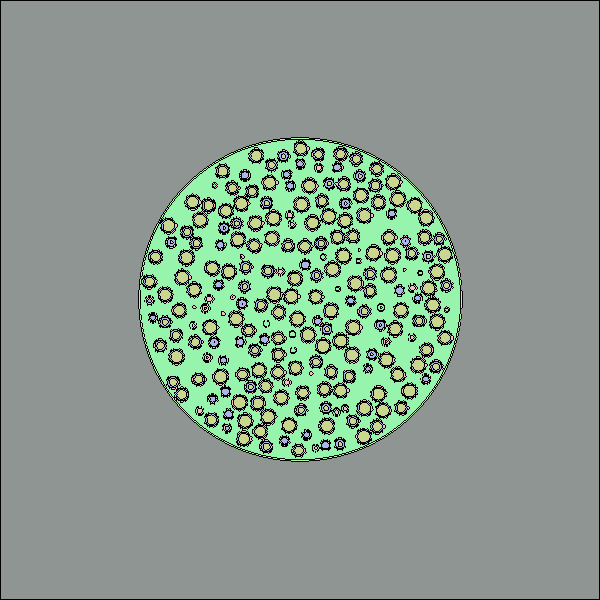
\includegraphics[width=\linewidth]{figures/FCM_geom1.png} 
			\caption{XY-plane view.}
			\label{fig:FCM_xy}
		\end{subfigure}
		\begin{subfigure}[t]{0.4\textwidth}
			\centering
			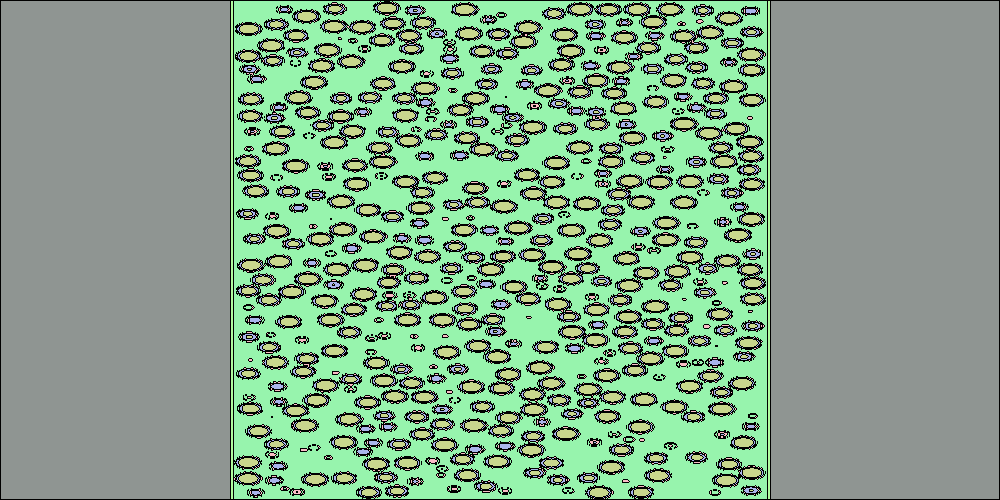
\includegraphics[width=\linewidth]{figures/FCM_geom2.png}
			\caption{YZ-plane view.}
			\label{fig:FCM_yz}
		\end{subfigure}
		\hfill
		\caption{FCM Serpent model geometry for different planes.}
		\label{fig:FCM}
	\end{figure}

	\begin{table}[htbp!]
		\centering
	    \caption{TRISO and Fuel Compact Characteristics.}
	    \label{tab:compact}
		\begin{tabular}{l|l|l}
		\hline
		Characteristic              & Value             & Reference/Assumption \\ \hline
		Fuel                        & UO$_2$ + UC$_{0.5}$O$_{1.5}$ (50/50\%)  & Section 1 of \cite{hawari_development_2018} \\
		Enrichment (average)        & 12.0 wt\%         & Section 1 of \cite{hawari_development_2018}  \\
		Kernel radius               & 400 $\mu$m        & Table 5 of \cite{hawari_development_2018}  \\
		Buffer thickness            & 75 $\mu$m         & Table 5 of \cite{hawari_development_2018}  \\
		IPyC thickness              & 35 $\mu$m         & Table 5 of \cite{hawari_development_2018}  \\
		SiC thickness               & 35 $\mu$m         & 36.7 $\mu$m in table 5 of \cite{hawari_development_2018}  \\
		OPyC thickness              & 20 $\mu$m         & Table 5 of \cite{hawari_development_2018}  \\
    	Kernel density              & 10.8 g/cm$^3$     & Table 5 of \cite{hawari_development_2018}  \\
		Buffer density              & 0.98 g/cm$^3$     & Table 5 of \cite{hawari_development_2018}  \\
		IPyC density                & 1.85 g/cm$^3$     & Table 5 of \cite{hawari_development_2018}  \\
		SiC density                 & 3.2  g/cm$^3$     & Table 5 of \cite{hawari_development_2018}  \\
		OPyC density                & 1.85 g/cm$^3$     & 1.86 g/cm$^3$ in table 5 of \cite{hawari_development_2018}  \\
		SiC Matrix density          & 3.2 g/cm$^3$      & Table 1 of \cite{hawari_development_2018}  \\
		Packing Fraction (average)  & 39.9 \%           & 40\% in Table 1 of \cite{hawari_development_2018}  \\
		Compact diameter            & 2.14 cm           & Fuel pin diameter is 2.17 cm in Section 1 of \cite{hawari_development_2018}  \\
		Helium gap                  & 0.01 cm           & The presence of a gap is an assumption. \\
		Compact length              & 4.0 cm            & Value chosen arbitrily to model the compact. \\ 
        \multirow{ 2}{*}{Helium density} & \multirow{ 2}{*}{2.0526 kg/m$^3$}  & Ideal gas density, T=700K, P=3 MPa. \\
                                    &                   & Section 5 of \cite{hawari_development_2018} \\
        Block graphite density      & 1.75 g/cm$^3$     & Density of grade H-451 Graphite \cite{gougar_prismatic_2010} \\ \hline

		\end{tabular}
	\end{table}

\subsection{Assemblies and full core}

Three different types assemblies make up the core, the fuel assembly, the control rod assembly, and a central assembly.
The central assembly has one 12 cm-diameter control rod.

The input file that models the fuel assembly and the control rod assembly are \textit{fuel\_block} and \textit{control\_block}, respectively, Figure \ref{fig:assemblies}.
The input file that describes the full core is \textit{fullcore}, Figure \ref{fig:full}.

Table \ref{tab:fuel} and \ref{tab:control} summarize the characteristics of the fuel and the control rod assemblies.
The same tables provide information on the assumptions made.
The rest of the assumptions are listed below:

\begin{itemize}
	\item \cite{hawari_development_2018} does not mention the height of the core. \cite{venneri_neutronic_2015} considers a reactor height of 2 meters. Our model considers 4 fuel assemblies stacked on top of each other, reaching a core height of 272 cm.
	\item \cite{hawari_development_2018} does not specify the height of the reflector. We assume a 20 cm bottom and top reflector thickness.
	\item The core counts with a radial reflector of graphite and another one of BeO.
	The radial reflector of graphite has a diameter of 248.62 cm and the reflector of BeO has a diameter of 268.62 cm\cite{hawari_development_2018}.
	The model considers diameters of 248 cm and 268 cm, respectively.

\end{itemize}

See Section \ref{sec:comments} for further discussion on the assumptions.

	\begin{figure}[htbp!]
		\centering
		\begin{subfigure}[t]{0.4\textwidth}
			\centering
			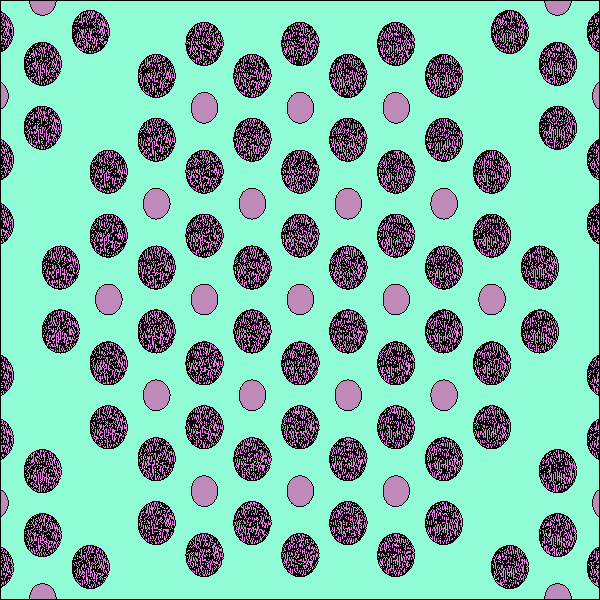
\includegraphics[width=\linewidth]{figures/fuel_block_geom1.png} 
			\caption{Fuel assembly serpent model.}
		\end{subfigure}
		\begin{subfigure}[t]{0.4\textwidth}
			\centering
			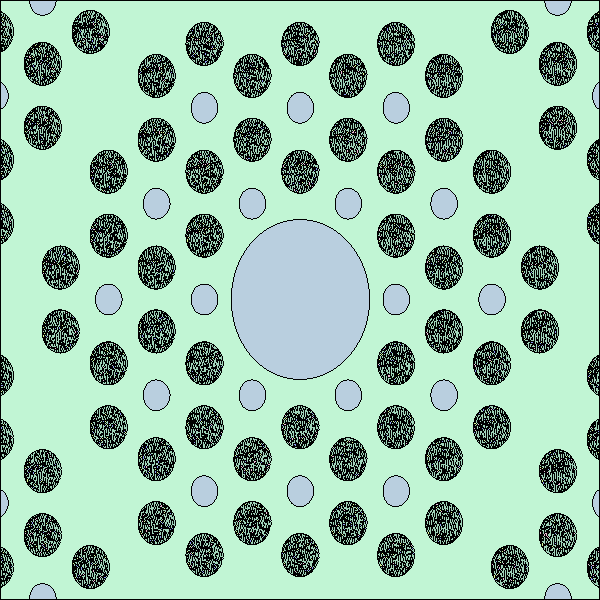
\includegraphics[width=\linewidth]{figures/control_block_geom1.png}
			\caption{Control rod assembly serpent model.}
		\end{subfigure}
		\hfill
		\caption{Different assemblies geometry.}
		\label{fig:assemblies}
	\end{figure}

	\begin{figure}[htbp!]
		\centering
		\begin{subfigure}[t]{0.4\textwidth}
			\centering
			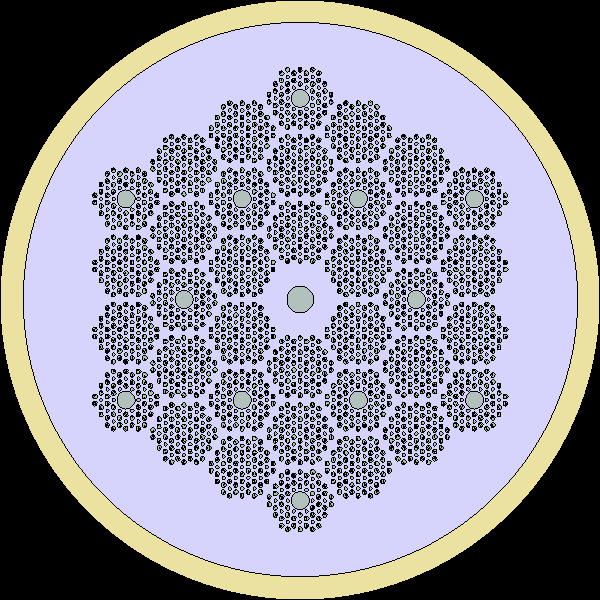
\includegraphics[width=\linewidth]{figures/fullcore_geom1.png} 
			\caption{XY-plane view.}
		\end{subfigure}
		\begin{subfigure}[t]{0.4\textwidth}
			\centering
			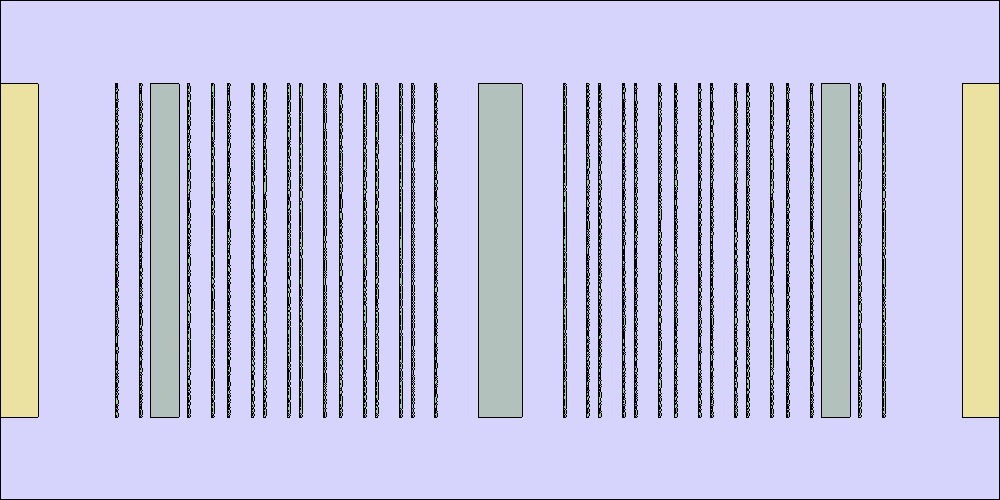
\includegraphics[width=\linewidth]{figures/fullcore_geom2.png}
			\caption{YZ-plane view.}
		\end{subfigure}
		\hfill
		\caption{Full core Serpent model for different planes.}
		\label{fig:full}
	\end{figure}

	\begin{table}[htbp!]
		\centering
	    \caption{Fuel Assembly Characteristics.}
	    \label{tab:fuel}
		\begin{tabular}{l|l|l}
		\hline
		Characteristic                   & Value         & Reference/Assumption \\ \hline
		Block pitch (flat-to-flat)       & 30 cm         & Section 1 of \cite{hawari_development_2018} \\
		Block graphite density           & 1.75 g/cm$^3$ & Density of grade H-451 Graphite \cite{gougar_prismatic_2010} \\
		Number of fuel holes             & 54            & Section 1 of \cite{hawari_development_2018} \\
		Fuel hole diameter               & 2.16 cm       & 2.17 cm in Section 1 of \cite{hawari_development_2018} \\
		Number of coolant holes          & 19            & Section 1 of \cite{hawari_development_2018} \\
		Coolant hole radius        		 & 1.54 cm       & 1.55 cm in Section 1 of \cite{hawari_development_2018} \\
		Flat-to-flat hexagonal lattice   & 6.4 cm        & Value infered. \\
		\multirow{ 2}{*}{Fuel length}    & \multirow{ 2}{*}{68 cm} & Fuel rod of 63.24 cm with top and bottom \\
                                         &               & graphite plugs of 2.38 cm. Section 1 of \cite{hawari_development_2018} \\ \hline
		\end{tabular}
	\end{table}

	\begin{table}[htbp!]
		\centering
	    \caption{Control Rod Assembly Characteristics.}
	    \label{tab:control}
		\begin{tabular}{l|l|l}
		\hline
		Characteristic                   & Value         & Reference/Assumption \\ \hline
		Block pitch (flat-to-flat)       & 30 cm         & Section 1 of \cite{hawari_development_2018} \\
		Block graphite density           & 1.75 g/cm$^3$ & Density of grade H-451 Graphite \cite{gougar_prismatic_2010} \\
		Number of fuel holes             & 48            & Section 1 of \cite{hawari_development_2018} \\
		Fuel hole diameter               & 2.16 cm       & 2.17 cm in Section 1 of \cite{hawari_development_2018} \\
		Number of coolant holes          & 18            & Section 1 of \cite{hawari_development_2018} \\
		Large coolant hole radius        & 1.54 cm       & 1.55 cm in Section 1 of \cite{hawari_development_2018} \\
		Flat-to-flat hexagonal lattice   & 6.4 cm        & Value infered. \\
		\multirow{ 2}{*}{Fuel length}    & \multirow{ 2}{*}{68 cm} & Fuel rod of 63.24 cm with top and bottom \\
                                         &               & graphite plugs of 2.38 cm. Section 1 of \cite{hawari_development_2018} \\ 
		Control rod diameter             & 8 cm          & Section 1 of \cite{hawari_development_2018} \\ \hline
		\end{tabular}
	\end{table}

\section{Results}

Table \ref{tab:results1} shows the results of the eigenvalue calculations in Serpent of the FCM and the full core.

Figure \ref{fig:results2} presents the variation of $k_{eff}$ and the mass of $U_{235}$ with the burn up.

For the depletion calculations, we consider a reactor power of 10 MW-th.

	\begin{table}[htbp!]
		\centering
	    \caption{$k_{eff}$ for different configurations.}
	    \label{tab:results1}
		\begin{tabular}{l|l}
		\hline
		             & $k_{eff}$ (analog)  \\ \hline
		FCM          & 1.53402 +/- 0.00084 \\ 
		fullcore     & 1.13582 +/- 0.00052 \\ \hline

		\end{tabular}
	\end{table}

%Depeltions calculations
	\begin{figure}[htbp!]
		\centering
		\begin{subfigure}[t]{0.4\textwidth}
			\centering
			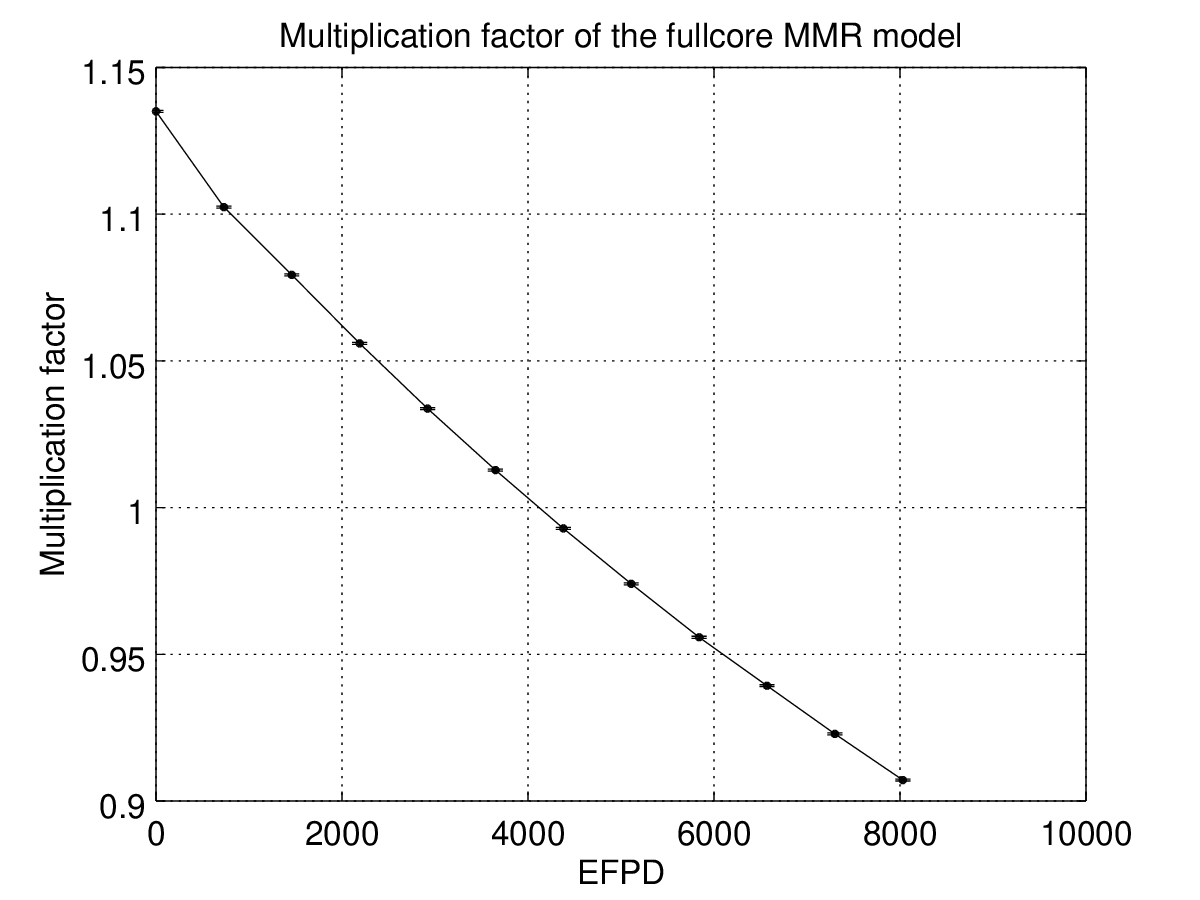
\includegraphics[width=\linewidth]{figures/Keff.png}
			\caption{$k_{eff}$ of the full core for different burn ups.}
		\end{subfigure}
		\begin{subfigure}[t]{0.4\textwidth}
			\centering
			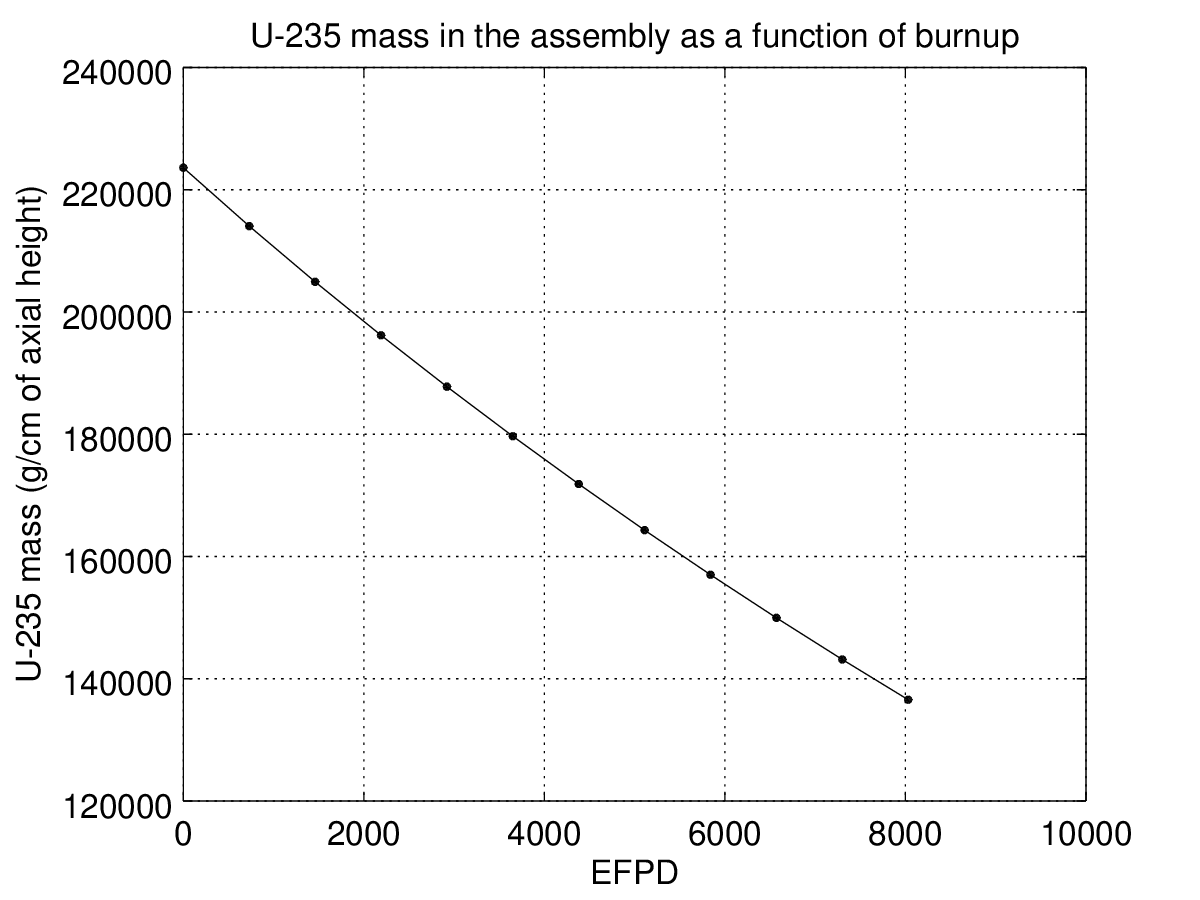
\includegraphics[width=\linewidth]{figures/mU235.png}
			\caption{$U_{235}$ mass of the full core for different burn ups.}
		\end{subfigure}
		\hfill
		\caption{Burnup calculation results.}
		\label{fig:results2}
	\end{figure}

\section{Comments}
\label{sec:comments}

This section discusses a few discrepancies between the adopted model and models from other documents.

The values for the TRISO particles are not equal to the values found in other documents such as \cite{venneri_neutronic_2015}, but are very close.

While \cite{venneri_neutronic_2015} uses a fuel compact of 0.7 cm of radius, \cite{hawari_development_2018} uses a fuel pin diameter of 2.17 cm. The model adopts a value of 2.16 cm.
\cite{venneri_neutronic_2015} uses a coolant hole of 0.4 cm-radius, and a 17 mm center to center distance hexagonal lattice.
Section 3 of the same document defines the core with graphite pancake-like blocks.
The blocks are 25 cm thick quarter disks with a diameter of 200 cm and a total length of 200 cm, surrounded by a 50 cm thick beryllium oxide reflectors.
The overall core assembly size is 300 cm in diameter and 300 cm in length.

\pagebreak
\bibliographystyle{plain}
\bibliography{bibliography}

\end{document}
